%% !TeX root = main.tex
\chapter{Binary Neural Networks (BNNs)}
\label{chapter:BNN}

\section{Overview}
\emph{Binary Neural Networks (BNNs)} are efficient neural network architectures that operate with binary weights and activations rather than full precision values as done in typical neural networks. Binary operations simplify computations by moving from higher precision arithmetic to bit-level operations. Binary operations provide significant advantages in terms of power, performance, and area. Yet, they have significantly less precision than floating point, fixed point, or integer representations.  

This chapter introduces BNNs, provides a basic understanding about how they function, and develops HLS code to implement a small BNN. The chapter begins by motivating the development of BNNs with a discussion of the benefits these networks provide with respect to computational efficiency and memory consumption. Next, the basic operations and concepts behind BNNs are explained to give an idea of how binary values are created and used within the network. Then, the chapter describes model inference and training, i.e., forward and backward propagation, and discuss how BNNs address the challenges that arise as a result of using only binary values. 

\begin{figure}[htbp]
\centerline{\includegraphics[scale = .75]{images/network.png}}
\caption{High-level depiction of a Binary Neural Network (BNN). Data is quantized to binary values making computation and storage more efficient~\cite{paperExplained}.}
\label{fig:network}
\end{figure}


\section{Motivation}

The development of BNNs is driven by the need for efficiency, particularly in resource-constrained environments. Floating-point precision provides precision, but also requires the significant computational resources and memory capacities for computation and parameter storage. Floating point is often too slow, too large, or even infeasible for small devices. BNNs drastically reduce the memory footprint and computational complexity by using binary values and bitwise operations, making them particularly well-suited for deployment in edge devices, IoT applications, and other scenarios where resources are limited. 

BNNs translate floating point operations to more efficient binary operations. We will show how the multiplications and additions can be replaced by XNOR and population count, which facilitates efficient forward and backward propagation. By swapping dot products with these more efficient bitwise operations, BNNs are faster, use fewer resources, and less power in FPGAs and other hardware implementations. 

Compare the 32-bit floating point values used in most deep neural networks to a single bit used in BNNs. 
The single bit (binary) representation uses 1/32 of the space required by the 32-bit representation making it 32 times more memory efficient. 
The same is true even for 32-bit integer values. %Further, bitwise operations require significantly less and faster logic than that necessary for floating point calculations. 
Binary operations are faster, use fewer resources, and less power than floating point operations. 
Such improved efficiency translates to accelerated inference times and enables BNNs to be used for applications making real-time decisions.

\section{Quantization}

As discussed Chapter~\ref{sec:number_representation}, numbers can be represented in many different ways. 
Quantization is the notion of mapping a larger set of values to a smaller set of values. 
Quantization can take many forms, and is very important for hardware optimization. 
For example, one could quantize a floating point number to a fixed point representation and get significant benefits in computation time, resource usage, and power consumption.
If the fixed point number was less than 32 total bits, there would also be storage/memory benefits.
A binary number represents the extreme of quantization.
It transforms a number to one of two possible values. 

The signum function is widely used in BNNs for quantization. The signum function maps a larger bit input number to binary number of -1 or +1 based on the sign of the input value. 
Calculating the signum function is computationally inexpensive, making it extremely hardware efficient.
For floating point numbers, this is solely a function of the sign bit, which is the most significant bit. 
Similarly, the most significant bit of an integer value indicates the sign of the integer in two's complement representation.
Thus, the signum function can be efficiently implemented in hardware with minimal resource usage.  

The mathematical definition of the signum function is:
$$
x^{b} = \text{sgn}(x) =
\begin{cases}
+1, & \text{if } x > 0 \\
-1, & \text{otherwise}
\end{cases}
$$
where $x^{b}$ denotes the binarized or quantized value of $x$.

\begin{figure}
\centering
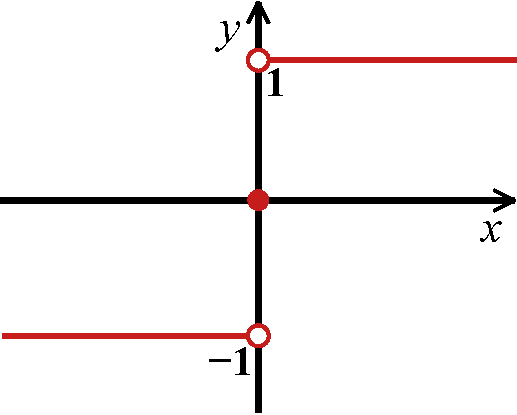
\includegraphics[width=.3\textwidth]{images/signum.pdf}
\caption{ A graphical representation of the signum function. Negative numbers are quantized to -1 and positive numbers are quantized to +1. The quantization is simple to implement in hardware as it only requires checking the sign bit of the input number. Source: Cronholm144, CC BY-SA 3.0, \url{https://commons.wikimedia.org/w/index.php?curid=2323348}.
}
\label{fig:signum}
\end{figure}

Consider two vectors $[10, -10, -5, 9, -8, 2, 3, 1]$ and $[12, -18, -13, -13, -14, -15, 11, 12].$ 
We can binarize these using the signum function to convert our values to -1 or +1 and obtain $[1, -1, -1, 1, -1, 1, 1, 1]$ and $[1, -1, -1, -1, -1, -1, 1, 1]$. This is shown in Figure~\ref{fig:signum-binarize}.

\begin{figure} 
\centering
\includegraphics[width=\textwidth]{images/signum-binarize.pdf}
\caption{ Using the signum function to binarize two vectors.
}
\label{fig:signum-binarize}
\end{figure}


%Then we perform both matrix multiplication (dot product) and XNOR with popcount and compare the results. Note that in order to use XNOR the values were first quantized to 0s and 1's. As depicted in the graphic on the next page, it is clear that both operations result in the same final output value of $3$.

%\begin{exercise}
%Can you guess why this may be the case? Think about how logical operation, specifically XNOR, could relate to multiplication.
%\end{exercise} 


\section{Binary Operations}
\label{sec:binary_operations}

Binary operations are much simpler to compute than floating point, integer, or fixed-point operations. Taking the previous two binarized vectors as an example, we can perform a binary dot product as shown in Figure~\ref{fig:binary-dot-product}.

\begin{figure}[h]
\centering
\includegraphics[width=.6\textwidth]{images/binary-dot-product.pdf}
\caption{ The dot product of the two binarized vectors from Figure~\ref{fig:signum-binarize}. The vectors are multiplied and the resulting vector is accumulated, i.e., reduced to a scalar.
} 
\label{fig:binary-dot-product}
\end{figure}

While much simpler to compute, the binary dot product is not quite ready for a hardware implementation. Digital hardware represents data as 0s and 1s, not -1s and +1s. Thus, we should translate or quantize the -1 and +1 values to 0s and 1s. This is done by mapping -1 to 1 and +1 to 0. Consider again the two vectors $[10, -10, -5, 9, -8, 2, 3, 1]$ and $[12, -18, -13, -13, -14, -15, 11, 12].$ 
The two binarized vectors then become $[0, 1, 1, 0, 1, 0, 0, 0]$ and $[0, 1, 1, 1, 1, 1, 0, 0]$.

\begin{exercise}
Another potential way to quantize/represent -1 and 1 would be 0 and 1. Why would one prefer the representation 1 and 0? Think about the conversion of negative and positive numbers to binary. Which way would require the least amount of logic? 
\end{exercise}

To perform the dot product of these two binary vectors, we can perform the following operations: quantize to 0,1, exclusive NOR of the resulting 0,1 quantization, and population count (popcount). These operations are much more efficient to implement in hardware than multiplication and addition.

The \emph{exclusive NOR (XNOR)} operation is a digital logic gate that acts as an exclusive or (XOR) operation followed by a NOT operation (inverter gate) . As seen in Figure~\ref{fig:xnor}, its output is “true” if the inputs are the same and “false” otherwise.  

\begin{figure}[h]
\centerline{\includegraphics[scale = .65]{images/xnor.png}}
\caption{XNOR logic gate and truth table. XNOR is used in BNNs to replace multiplication operations.}
\label{fig:xnor}
\end{figure}

In the context of BNNs, the XNOR operation is applied element-wise between binary inputs to a layer and binary weights to perform a multiplication. The resulting binary output indicates whether the input and weight have the same or different sign. The output of the XNOR operation is 1 when the result of the -1,1 multiplication is 1 and 0 when the result is -1.

\begin{figure}[h]
\centering
\includegraphics[width=.6\textwidth]{images/xnor-binary-multiplication.pdf}
\caption{ Comparing the -1,1 binary multiplication with the XNOR operation. The first two columns are the inputs and the last column is the output. The XNOR operation quantizes the -1,1 to 1,0 and then performs the XNOR on the 0,1 binary values. The result of the XNOR operation is the number of 1 in the -1,1 multiplication.}
\label{fig:xnor-binary-multiplication}
\end{figure}

Figure~\ref{fig:xnor} compares the binary multiplication of -1 and +1 with the XNOR operation when -1 is mapped to 1 and +1 is mapped to 0. The left table shows the results of the -1,1 binary multiplication. The right table first quantizes the -1,1 input values to 1,0. Then it performs the XNOR operation on the 0,1 binary values. The results of the XNOR operations is equal to the number of 1 in the -1,1 multiplication. Note this is different than if we performed a reverse mapping/quantization from 0,1 to 1,-1. 





%It was mentioned previously that using -1 and 1 as the binary values in a BNN was preferred over 0 and 1. The reason for this lies in the XNOR operation. Consider two binary inputs $A \in \{0,1\}$ and $B \in \{0,1\}$ and perform the XNOR operation on these values. Then, map 0 to -1 and 1 to +1 so that $A \in \{-1,+1\}$ and $B \in \{-1,+1\}$ and perform multiplication on these values.

%\newpage

%\begin{figure}[htbp]
%\centerline{\includegraphics[scale = .65]{images/comparison.png}}
%\label{fig:comparison}
%\end{figure}




\subsection{Population Count}
Next we perform the reduction or summation of the multiplied results, which, along with the multiplication, is necessary to complete the dot product operation.
The population count (popcount) operation counts the number of ``set'' bits (i.e., those equal to 1) in a binary vector. Popcount is a common operation in many processor architectures. And it is very efficient to implement in hardware.

Figure~\ref{fig:binary-0-1-dot-product} shows the dot product of the two binarized vectors from Figure~\ref{fig:signum-binarize}, but with the input -1 and +1 values quantized to 1 and 0. The multiplication is performed using XNOR, and the summation is performed using popcount.

\begin{figure}[h]
\centering
\includegraphics[width=.6\textwidth]{images/binary-0-1-dot-product.pdf}
\caption{ The dot product of the two binarized vectors from Figure~\ref{fig:signum-binarize}. This is similar to Figure~\ref{fig:binary-dot-product} except the binarization is to 0 and 1 instead of 1 and -1. The vectors are multiplied and the resulting vector is accumulated, which can be done with the popcount operation. The dot product here represents the total number of 1 outputs in the -1,1 multiplication vector.
} 
\label{fig:binary-0-1-dot-product}
\end{figure}

The result of the XNOR and popcount dot product is $6$. Compare this with the result of the -1,1 dot product from Figure~\ref{fig:binary-dot-product}, which is $4$. It should not be too surprising that the results are different. After all, the result of the XNOR operation is either 0 or 1, so its summation will always be non-negative. While the result of the -1,1 multiplication is either -1 or +1, so its summation can be negative. 

However, there is a simple relationship between the two results. To understand their relationship, let's define some terms. First, let $N$ be the number of elements in the vector, i.e., the vector length. Let $n$ be the number of unset bits in the 0,1 binary vector. And let $p$ be the number of set bits in the 0,1 binary vector.

We know that $p+n = N$, i.e., the number of set and unset bits in the vector is equal to the total number of elements in the vector or the vector length.

The summation of the 0,1 vector is $p$. 

Recall that a set bit (1) in the 0,1 vector means that both the input values are the same in the -1,1 multiplication, i.e., the input values are -1*-1 or 1*1 and both results in -1,1 multiplication is 1. An unset bit (0) means that the input values are different in the -1,1 multiplication, i.e., the input values are either -1*1 or 1*-1, which are both equal to -1 in the -1,1 multiplication. Thus, the summation of the -1,1 vector is $p - n$ where $p$ is the total set bits and $n$ is the total unset bits.


The summation of the -1,1 vector, which we denote as $\sum_{-1,1} = p-n$. We can rewrite $p+n = N$ as $n = N - p$ and substitute that back into the $\sum_{-1,1}$ equation to get:\\
\begin{equation}
\sum_{-1,1} = p - (N - p) = 2p - N
\label{eq:sum_minus1_1}
\end{equation}

Equation~\ref{eq:sum_minus1_1} defines the relationship between the summation of the -1,1 vector ($\sum_{-1,1}$) and the summation of the 0,1 vector ($\sum_{0,1}$). We can take the result of the $\sum_{0,1}$ in Figure~\ref{fig:binary-0-1-dot-product}, which is $6$, and plug it into Equation~\ref{eq:sum_minus1_1} to get the result of the $\sum_{-1,1}$. Thus, $\sum_{-1,1} = 2*6 - 8 = 4$, which matches the result from Figure~\ref{fig:binary-dot-product}.




%\subsection{XNOR and Popcount for Matrix Multiplication}
%In combination, XNOR and popcount operations can replace normal MAC (multiply-accumulate) operations in BNNs. Below is the general formula for multiplying two binary vectors $A$ and $B$ using XNOR and popcount.
%
%\begin{equation}
%    A \cdot B = sum - (N-sum) = 2*sum - N 
%\end{equation}
%
%where, 
%\begin{equation}
%sum = popcount(\overline{A \oplus B}) \\
%\end{equation}\\
%
%
%Here, $sum$ is the number of +1's in the dot product result, $N$ is the total number of bits of the XNOR result, and $N-sum$ is the number of -1's in the dot product result. \\
%
%\subsubsection{Example}
%Let's take a look at an example to convince you of the equivalence of matrix multiplication and the XNOR popcount operations. \\
%
%Consider two input vectors $[10, -10, -5, 9, -8, 2, 3, 1, -11]$ and $[12, -18, -13, -13, -14, -15, 11, 12, 13].$ We first binarize these using the sign function (defined in the next section) to convert our values to -1 or +1 and obtain $[1, -1, -1, 1, -1, 1, 1, 1, -1]$ and $[1, -1, -1, -1, -1, -1, 1, 1, 1]$. Then we perform both matrix multiplication (dot product) and XNOR with popcount and compare the results. Note that in order to use XNOR the values were first quantized to 0s and 1's. As depicted in the graphic on the next page, it is clear that both operations result in the same final output value of $3$. \\
%
%\begin{figure}[htbp]
%\centerline{\includegraphics[scale = .50]{images/example.png}}
%\label{fig:examplebnn}
%\caption{Example of normal MAC vs XNOR and popcount operations.}
%\end{figure}
%
%\newpage
%
%\section{Binarization of the Network}
%In order to achieve the benefits of using binary values in-place of floating point values %discussed above, we need a way to ``binarize''
% our network. There are two binarization functions that can be used to convert the neural network's floating point values into binary values of -1 or 1. 
%
%The first is the deterministic signum or sign function which, as the name suggests, maps real-values to -1 or 1 based on their sign. The sign function is defined as:
%
%\begin{equation}
%x^{b} = Sign(x) =
%    \begin{cases}
%        +1 & \text{if } x \geq{0} \\
%        -1 & \text{otherwise }
%    \end{cases}
%\end{equation}
%
%where $x^{b}$ is the binarized weight or activation and x is the original floating point %value. 
%\newpage
%
%The second binarization function is stochastic and is defined as:
%
%\begin{equation}
%x^{b} = Sign(x) =
%    \begin{cases}
%        +1 & \text{with probability} p = \sigma(x) \\
%        -1 & \text{with probability } 1-p
%    \end{cases}
%\end{equation}
%
%where $\sigma$ is:
%\begin{equation}
%    \sigma (x)= max(0, min(1, \frac{x+1}{2})
%\end{equation}
%\\
%
%Although the stochastic binarization can be esspecially effective in dealing with variability in data as compared to the deterministic case, it is harder to implement as it requires the hardware to generate random bits when quantizing. As a result, the deterministic sign function is more often used in practice and is what should used in your BNN project. 
%
%\begin{exercise}
%What classification tasks would perform better with stochastic binarization? Could we %achieve the same performance with deterministic binarization if we add more layers?
%\end{exercise}
%
%\newpage

\section{Forward Propagation}
Recall that in deep learning, forward propagation refers to model inference. That is, given an input, use the model's learned parameters to predict the output. For BNNs, the forward pass is similar to that of any typical deep neural networks architecture with the exception that all weights and activations are binarized to either -1 or +1. 

\subsection{General BNN Forward Propagation Psuedo Code}
The pseudo code for forward propagation of a BNN is shown below. Note that the superscript $b$ on a variable indicates that that variable is binarized. 

For layers $1$ through $L$, the weights are first binarized (and quantized) using the sign function. This step is only necessary during training, however, since once the model is fully trained only the binary weights will be stored. Then, our binary activations from the previous layer and binary weights are multiplied using the XNOR and popcount operations resulting in a non-binary sum. Following this, batch normalization is applied, if necessary, with parameters $\theta_k$. If it is not the last layer of the network, then activations are once again binarized and the process is repeated. 

\begin{figure}[htbp]
\centerline{\includegraphics[scale = .65]{images/forward.png}}
\caption{Pseudo code for BNN forward propagation}
\label{fig:forward}
\end{figure}

\subsection{BNN Forward Propagation Implementation using XNOR and Popcount}
Below you will find a Python implementation for a BNN forward pass, i.e., BNN inference. This network takes a 28x28 MNIST image as input and classifies the digit depicted in the images from 0-9. There are three fully connected layers to this BNN, with each implementing the process described in the pseudo code above: (1) Inputs to each layer (i.e., activations from the previous layer) are binarized and quantized. (2) These inputs are then multiplied with the binary weights using XNOR + popcount. (3) The output is fed to the next layer or used to make the final prediction. 

The model is already trained and the weights for each of the layers are stored in``fc1w\_qntz'', ``fc2w\_qntz'', ``fc3w\_qntz''. These are binary weights stored as 


\begin{python}
def feed_forward_quantized(self, input):
    #param input: MNIST sample input
    
    # layer 1
    X0_input = self.quantize(self.sign(self.adj(input)))
    layer1_output = self.matmul_xnor(X0_input, self.fc1w_qntz.T)
    layer1_activations = (layer1_output * 2 - 784)

    # layer 2
    layer2_input = self.sign(layer1_activations)
    layer2_quantized = self.quantize(layer2_input)
    layer2_output = self.matmul_xnor(layer2_quantized, self.fc2w_qntz.T)
    layer2_activations = (layer2_output * 2 - 128)

    # layer 3
    layer3_input = self.sign(layer2_activations)
    layer3_quantized = self.quantize(layer3_input)
    layer3_output = self.matmul_xnor(layer3_quantized, self.fc3w_qntz.T)

    final_output = (layer3_output * 2 - 64)
    A = np.array([final_output], np.int32)
        
    return A

\end{python}

\subsection{BNN Forward Propagation Implementation Using MAC}

For comparison, we have included a BNN forward propagation implementation using multiply and accumulate (MAC) rather than the XNOR and popcount introduced above. We hope it is now clear that this implementation is significantly more costly to implement in hardware. \\

\begin{python}
def feed_forward(self, input):
     """This BNN using normal MAC.
    """
    # layer 1
    X0_q = self.sign(self.adj(input))
    X1 = np.matmul(X0_q, self.fc1w_q.T)

    # layer 2
    X1_q = self.sign(X1)
    X2 = np.matmul(X1_q, self.fc2w_q.T)

    # layer 3
    X2_q = self.sign(X2)
    X3 = np.matmul(X2_q, self.fc3w_q.T)

    return X3
\end{python}


\subsection{BNN Forward Propagation Implementation in C++, Quantized}

Below we have included the feed\_forward\_quantized function in C++, for use in HLS. 
Firstly, we establish our helper functions. These include a function for executing the XNOR operation, another for the sign operation, a function for the quantize operation, and one for conducting matrix multiplication utilizing the XNOR operation. The primary feed-forward function is denoted as feed\_forward\_quantize(), designed for a two-layer Binary Neural Network (BNN). It is important to observe that flattened weight matrices are employed, and the dimensions of the original square matrices are supplied as parameters.

\begin{lstlisting}
#include <iostream>
#include <cmath>

int XNOR(int a, int b) {
    return (a == b) ? 1 : 0;
}
void matmul_xnor(int* A, int* B, int* res, int rowsA, int rowsB, int colsB) {
    for (int x = 0; x < colsB; ++x) {
        int cnt = 0;
        for (int y = 0; y < rowsA; ++y) {
            cnt += XNOR(A[y], B[y * colsB + x]);
        }
        res[x] = cnt;
    }
}
int quantize(int x) {
    return (x == 1) ? 0 : 1;
}
int sign(int x) {
    return (x > 0) ? 1 : -1;
}

void feed_forward_quantized(int* X, int* w1, int* w2, 
                            int X_size, 
                            int rowsW1, int colsW1, 
                            int rowsW2, int colsW2,
                            int* layer1_activations, int* layer2_activations) {

    // ********** Layer 1 **********
    // Quantize inputs
    int X0_input[X_size];
    for (int i = 0; i < X_size; ++i) {
        X0_input[i] = quantize(sign(X[i]));
    }
    // Perform matrix multiplication with W1 using XNOR
    matmul_xnor(X0_input, w1, layer1_activations, X_size, rowsW1, colsW1);
    for (int i = 0; i < colsW1; ++i) {
        layer1_activations[i] = (layer1_activations[i] * 2 - X_size);
    }
    // ********** Layer 2 **********
    // Quantize layer 1 activations
    int layer2_quantized[colsW1];
    for (int i = 0; i < colsW1; ++i) {
        layer2_quantized[i] = quantize(sign(layer1_activations[i]));
    }
    // Perform matrix multiplication with W2 using XNOR
    matmul_xnor(layer2_quantized, w2, layer2_activations, colsW1, rowsW2, colsW2);
    for (int i = 0; i < colsW2; ++i) {
        layer2_activations[i] = (layer2_activations[i] * 2 - colsW1);
    }
    // final output is layer2_activations
}

int main() {
    // Example usage:
    int input[] = { 1, 1 };
    int W1[] = {1, 1, 1, 1};
    int W2[] = {1, 0, 1, 1, 1, 0};
    int X_size = 2;
    int rowsW1 = 2;
    int colsW1 = 2;
    int rowsW2 = 2;
    int colsW2 = 3;
    int layer1_activations[colsW1];
    int layer2_activations[colsW2];

    feed_forward_quantized(input, W1, W2, X_size, rowsW1, colsW1, rowsW2, colsW2,
                            layer1_activations, layer2_activations);
    return 0;
}
\end{lstlisting}





\section{Back Propagation}

Backpropagation (short for ``backwards propagation of errors'') is a fundamental algorithm used to train supervised learning algorithms - BNNs being one of them. At the end of the forward pass (forward propagation), the network computes the loss (error) by comparing its outputs to the ground truth values using a loss function such as mean squared error for regression tasks or cross-entropy for classification tasks. The algorithm then calculates the gradient of the loss function with respect to each weight in the network by applying the chain rule.

\begin{exercise}
Can you think of any issue with taking the gradient here? Remember in forward propagation, we used Sign(x) to binarize weights. What does the derivative look like for this function?
\end{exercise} 

\subsection{Gradient Descent Update Rule}

Backpropagation gets its name from the fact that this chain rule process starts at the output layer and works backward through the network. The weights are then updated to minimize the loss (error) function, shown below with W the weight to update, J the loss function, and $\alpha$ the learning rate. This update process is called gradient descent.

\begin{figure}[htbp]
\centerline{\includegraphics[scale = .65]{images/grad_decent.png}}
\caption{Gradient descent update rule.}
\label{fig:grad_descent}
\end{figure}

This process of forward and backward propagation is repeated for many iterations, updating the weights of the network each time to minimize the loss function. Below is a graphical depiction of BNN training.

\begin{figure}[htbp]
\centerline{\includegraphics[scale = .35]{images/network_overview.png}}
\caption{Overview of BNN training, with an emphasis on forward and backward propagation.}
\label{fig:network_overview}
\end{figure}
Remember that weights are binarized in forward propagation. Recall the signum function used for deterministic binarization (see Figure~\ref{fig:signum}). Note that the derivative of the signum function is zero almost everywhere, which makes it seem incompatible with the backward propagation method described above, where all gradients would equal zero. So how do BNNs get around this issue?

%\begin{figure}
%\centerline{\includegraphics[scale = .15]{images/sign.png}}
%\caption{Plot of sign(x) for deterministic binarization. Note that the derivative of sign(x) with respect to x is zero for nearly all x.}
%\label{fig:sign}
%\end{figure}


\subsection{Straight-Through Estimator}

Rather than use the analytical gradient of the loss with respect to the weights, we will calculate an estimate. In the context of backpropagation in BNNs, we will call this a straight through estimator (STE). In STEs, you set the incoming gradients to a threshold function equal to its outgoing gradients, disregarding the gradient of the threshold function itself. The figure below shows one layer of a BNN with Sign(x) as the activation function. Note that the top row is depicting a forward pass where Z are the incoming weights and Y are the outgoing weights (Y = Sign(Z)). The bottom row is depicting a backward pass on weights with respect to a loss function, L. On the backward pass, let \( g_Y = \frac{\partial L}{\partial Y} \) be the incoming derivative and let \( g_Z = \frac{\partial L}{\partial Z} \) be the analytical derivative (which would be 0 based on the analysis above). The STE computes \( g_Z \) to be \( g_Y \times \mathbb{1}_{\lvert Z \rvert \leq 1} \) where \( \times \) is element-wise multiplication with the indicator function. This is a difficult concept to grasp, but informally, this STE allows the binarization function to act as the identity function in the region around the current point (equivalent to using hard tanh function). %\\\\



\begin{figure}[h]
    \centering
    \begin{minipage}{0.45\textwidth}
        \centering
        \includegraphics[width=\textwidth]{images/STE.png}
        \caption{Zoomed-in look at one layer of BNN during training, showing use of STE during backpropagation.}
    \end{minipage}\hfill
    \begin{minipage}{0.37\textwidth}
        \centering
        \includegraphics[width=\textwidth]{images/hard_tanh.png}
        \caption{STE estimation of Sign function, as hard tanh function.}
    \end{minipage}
\end{figure}


% \begin{figure}[htbp]
% \centerline{\includegraphics[scale = .75]{STE.png}}
% \caption{Zoomed-in look at one layer of BNN during training, showing use of STE during backpropagation.}
% \label{fig2}
% \end{figure}

% \begin{figure}[htbp]
% \centerline{\includegraphics[scale = .55]{hard_tanh.png}}
% \caption{STE estimation of Sign function, as hard tanh function.}
% \label{fig2}
% \end{figure}

\newpage

\subsection{Backpropagation Pseudo Code}

The pseudo code for backward propagation of a BNN is shown below. We have also defined some important terms. In short, for each layer (except the last), we apply straight through estimation. We then perform a backwards pass for BatchNorm and calculate the estimated gradients of the weights with respect to the loss, and apply activation (the transpose step). In the second for loop, the weights are updated via gradient descent, and the gradients are passed left through the network.



\begin{itemize}
    \item C - loss function
    \item L - number of layers
    \item g - gradient (partial derivative)
    \item $s_k$ - activations before BatchNorm
    \item $a_k$ - activations after BatchNorm
    \item W - weight matrix
    \item superscript 'b' refers to a 'binarized' form of the variable
    \item $\theta$ - BatchNorm parameters
    \item $\eta$ - learning rate
\end{itemize}

\begin{figure}
\centerline{\includegraphics[scale = .35]{images/backprop_code.png}}
\centerline{\includegraphics[scale = .50]{images/backprop_2.png}}
\caption{Pseudo code for BNN backward propagation}
\label{fig:backprop2}
\end{figure}



\section{Conclusion}
BNNs are an efficient operation used in many resource-constrained computing devices. An input to a BNN is a list (x vector). Let's say our goal is to predict the y. The network, having taken in a vector x, will perform the following operations to predict y (referred to as inference in neural networks). During the forward pass, the input data is processed through the network's layers, using the trained binary weights and activations. In BNNs, the standard dot product in the neurons is replaced by XNOR and popcount operations. These operations are much more efficient than floating-point multiplications and additions. At each layer, after the XNOR and bitcount operations, an activation function is applied (signum). BNNs can use batch normalization to stabilize and speed up training. During inference, the learned parameters from batch normalization are used to normalize the activations. If the network includes pooling layers, convolutional layers, or other types of layers, these operate in a similar manner to their counterparts in traditional neural networks, but they are adapted to work with binary values. Finally, at the output layer, we receive our value for y (regression) or pass the final vector through typically a soft max (classification).

The key advantage of BNNs is that they require significantly less computational power and memory than traditional neural networks, making them well-suited for resource-constrained environments like mobile devices or embedded systems. However, the trade-off is that the binarization of weights and activations can lead to a loss in model accuracy, especially for complex tasks. In simple tasks such as number recognition, the BNN performs well, although requiring more layers than a full-precision NN. For complex tasks such as high-resolution image classification and natural language processing, the lower expressiveness of the BNN may struggle to recognize complex patterns.


%\nocite{bnn1, vid1, vid2, vid3, vid4, vid5, vid6}
% \nocite{stanford} \nocite{paper_explained} \nocite{review}

% \begin{thebibliography} {00}
% \bibitem{slides1} “Binary Neural Networks.” Lecture, n.d. https://docs.google.com/presentation/d/10lVe51Nh7w\_
% qmhlYheaYP1b8q6iOsutZ/edit#slide=id.p1. 
% \bibitem{bnn1}Courbariaux, Matthieu, Itay Hubara, Daniel Soudry, Ran El-Yaniv, and Yoshua Bengio. "Binarized neural networks: Training deep neural networks with weights and activations constrained to+ 1 or-1." arXiv preprint arXiv:1602.02830 (2016).
% \bibitem{vid1} EE545 (Week 10) “Binary Neural Networks” (Part I). YouTube. YouTube, 2020. https://www.youtube.com/watch?v=5K6ko3H\_ePg&amp;list=PLC89UNusI0eSBZhwHlGauwNq
% VQWTquWqp&amp;index=23&amp;t=338s. 
% \bibitem{vid2} EE545 (Week 10) “Binary Neural Networks” (Part II). YouTube. YouTube, 2020. https://www.youtube.com/watch?v=LcECmeFqbrI&amp;list=PLC89UNusI0eSBZhwHlGauwNq
% VQWTquWqp&amp;index=24. 
% \bibitem{vid3} EE545 (Week 10) “Binary Neural Networks” (Part III). YouTube. YouTube, 2020. https://www.youtube.com/watch?v=RC\_8bPv0uhM&amp;list=PLC89UNusI0eSBZhwHlGauwNq
% VQWTquWqp&amp;index=25. 
% \bibitem{vid4} EE545 (Week 10) “Binary Neural Networks” (Part IV). YouTube. YouTube, 2020. https://www.youtube.com/watch?v=P6sD8lI61Uk&amp;list=PLC89UNusI0eSBZhwHlGauwNq
% VQWTquWqp&amp;index=26. 
% \bibitem{vid5}EE545 (Week 10) “Binary Neural Networks” (Part V). YouTube. YouTube, 2020. https://www.youtube.com/watch?v=rHa0-mG5SuM&amp;list=PLC89UNusI0eSBZhwHlGauwNq
% VQWTquWqp&amp;index=27. 
% \bibitem{vid6} EE545 (Week 10) “Binary Neural Networks” (Part VI). YouTube. YouTube, 2020. https://www.youtube.com/watch?v=z8CclU5wKuY&amp;list=PLC89UNusI0eSBZhwHlGauwNq
% VQWTquWqp&amp;index=28. 
% \bibitem{stanford} Lin, Fang. Rep. XNOR Neural Networks on FPGA. CS231n: Deep Learning for Computer Vision, n.d. http://cs231n.stanford.edu/reports/2017/pdfs/118.pdf. 
% \bibitem{gpt} Ludvigsen, Kasper Groes Albin. “The Carbon Footprint of GPT-4.” Medium, July 18, 2023. https://towardsdatascience.com/the-carbon-footprint-of-gpt-4-d6c676eb21ae#:~:text=The\%20electricity\%20consumption\%20of\%20GPT\%2D4&amp;text=According\%20
% to\%20unverified\%20information\%20leaks,8\%20\%3D\%203\%2C125\%20servers\%20were\%20needed. 
% \bibitem{paper explained}Natsu. “Paper Explanation: Binarized Neural Networks: Training Neural Networks with Weights and Activations Constrained to +1 or −1.” Mohit Jain, August 16, 2018. https://mohitjain.me/2018/07/14/bnn/.
% \bibitem{slides2} "Neural Network.” Lecture, n.d. https://docs.google.com/presentation/d/1oC1Z\_LzzlGMdDCFpC
% 9rp6U2udwSpCaj-/edit#slide=id.p1. 
% \bibitem{medium} Ojha, Vikas Kuma. “Binary Neural Networks: A Game Changer in Machine Learning.” Web log. Geek Culture (blog). Medium, February 19, 2023. https://medium.com/geekculture/binary-neural-networks-a-game-changer-in-machine-learning-6ae0013d3dcb. 
% \bibitem{review}Yuan, Chunyu, and Sos S. Agaian. "A comprehensive review of binary neural network." Artificial Intelligence Review (2023): 1-65.

% \end{thebibliography}


% \nocite{*}
% \bibliographystyle{abbrv}
% \bibliography{ref}




% \end{document}


